
\documentclass[a4paper,12pt]{article}
\usepackage{graphicx}
\usepackage[table,xcdraw]{xcolor}
\usepackage{geometry}
\usepackage{float}
\usepackage[colorlinks=false, hidelinks]{hyperref}
\usepackage{fancyhdr}% For page numbering
\geometry{top=1in,bottom=1in,left=1in,right=1in}
\usepackage{listings}
\usepackage{xcolor}
\usepackage{hyperref}
\pagestyle{empty}

\usepackage{listings}
\usepackage{xcolor}

% Solarized color scheme
\definecolor{solarized-base03}{HTML}{002B36}
\definecolor{solarized-base02}{HTML}{073642}
\definecolor{solarized-base01}{HTML}{586E75}
\definecolor{solarized-base00}{HTML}{657B83}
\definecolor{solarized-base0}{HTML}{839496}
\definecolor{solarized-base1}{HTML}{93A1A1}
\definecolor{solarized-base2}{HTML}{EEE8D5}
\definecolor{solarized-base3}{HTML}{FDF6E3}
\definecolor{solarized-yellow}{HTML}{B58900}
\definecolor{solarized-orange}{HTML}{CB4B16}
\definecolor{solarized-red}{HTML}{DC322F}
\definecolor{solarized-magenta}{HTML}{D33682}
\definecolor{solarized-violet}{HTML}{6C71C4}
\definecolor{solarized-blue}{HTML}{268BD2}
\definecolor{solarized-cyan}{HTML}{2AA198}
\definecolor{solarized-green}{HTML}{859900}

% Python listing style
\lstdefinestyle{pythonSolarized}{
    language=Python,
    backgroundcolor=\color{solarized-base3},
    basicstyle=\ttfamily\small\color{solarized-base00},
    keywordstyle=\color{solarized-blue}\bfseries,
    stringstyle=\color{solarized-cyan},
    commentstyle=\color{solarized-base1}\itshape,
    numberstyle=\color{solarized-base1},
    identifierstyle=\color{solarized-base00},
    emphstyle=\color{solarized-green},
    breaklines=true,                % Enable line breaking
    breakatwhitespace=false,        % Break even in the middle of words
    postbreak=\mbox{\textcolor{solarized-orange}{$\hookrightarrow$}\space}, % Indicator for wrapped lines
    frame=single,                   % Draw a frame around the code
    rulecolor=\color{solarized-base2},
    numbersep=5pt,                  % Space between numbers and code
    xleftmargin=15pt,               % Margin for code
    xrightmargin=15pt,
    showstringspaces=false          % Don't show spaces in strings
}
\begin{document}

\begin{center}
    \textbf{\large{Lab Report: Unit Testing Report}}\\
    \vspace{0.2cm}
    \textbf{Course Title: Software Engineering \& ISD Lab}\\
    \vspace{0.2cm}
    \textbf{Course Code: CSE-404}\\
    \vspace{0.2cm}
    \textbf{4\textsuperscript{th}Year 1\textsuperscript{st}Semester Examination 2023}\\
    \vspace{0.5cm}
    \textbf{Date of Submission: \today}\\

    \vspace{1.5cm}
    
\includegraphics[width=0.35\textwidth]{images/logo.png}\\ % Replace 'logo.png' with the correct path if you have the university logo image
    \vspace{1cm}

    \textbf{Submitted to}\\
    \vspace{0.2cm}
    \textbf{\href{https://juniv.edu/teachers/musfique.anwar}{Dr. Md Musfique Anwar}}\\
    {Professor}\\
    \vspace{0.2cm}
    \textbf{\href{https://juniv.edu/teachers/hkabir}{Dr. Md. Humayun Kabir}}\\
    {Professor}\\


    \vspace{1cm}

    \begin{table}[h!]
        \centering
        \arrayrulecolor{black}
        \begin{tabular}{|c|c|c|c|}
            \hline
            \rowcolor[HTML]{2F4F4F} % Changed header background color to dark slate gray
            {\color[HTML]{FFFFFF}\textbf{Sl}}& {\color[HTML]{FFFFFF}\textbf{Class Roll}}& {\color[HTML]{FFFFFF}\textbf{Exam Roll}}& {\color[HTML]{FFFFFF}\textbf{Name}}\\ \hline
            \rowcolor[HTML]{B0E0E6}
            \textbf{1}& \textbf{408} & \textbf{202220} & \textbf{Sudipta Singha} \\ \hline
       
        \end{tabular}
    \end{table}

    \vspace{1cm}

    Department of Computer Science and Engineering\\
    Jahangirnagar University\\
    Savar, Dhaka, Bangladesh\\
\end{center}

\newpage

\tableofcontents

\newpage
\pagestyle{fancy}
\fancyhf{}
\fancyfoot[C]{\thepage} % Page number in the center of the footer
\section{Introduction}
Unit testing is a software development practice focused on testing individual units or components of a program
to ensure they function as intended. A “unit” is typically the smallest testable part of an application, such
as a function or method. By isolating each part of the program, developers can confirm that each unit behaves
correctly and contributes to the overall system’s reliability. Unit testing is widely regarded as a
cornerstone of modern software development practices.
\section{What is Unit Testing}
Unit testing involves writing specific tests for individual functions or methods in a codebase. These tests
are typically automated and verify that a given input to a unit produces the expected output..
\section{Example}
In the project where we developed  Jahangirnagar University Medical Center Management System, we are involved
in implementing various feature. I implemented \\
\textbf{Features}
\begin{enumerate}
    \item Create Account
    \item Dispense medicine to patients
    \item Update Stock information
\end{enumerate}
To test the features we have implemented , We have used django built-in unit testing tool. \\
\textbf{Feature}
\begin{itemize}
    \item Integration with unittest
    \item Test Database
    \item Client for Simulating Requests
    \item Fixtures
    \item Assertions
\end{itemize}
The reaseon we choose django unit testing as testing tool for our project is because of its Advantages \\
\textbf{Advantages}
\begin{itemize}
    \item Integration with Django
    \item Comprehensive Testing Tools
    \item Automatic Test Discovery.
\end{itemize}
\subsection{Create Account}
\textbf{Create Account Code}
\lstset{style=pythonSolarized}
\begin{lstlisting}
def register(request):
    """Handle user registration.

    This function processes registration requests, validates the user input,
    and saves the new user if valid. If the registration is successful,
    it redirects the user to the unapproved page.

    Args:
        request: The HTTP request object.

    Returns:
        HttpResponse: The rendered registration page or a redirect to the
            unapproved page.
    """
    if request.method == "POST":
        form = UserRegistrationForm(request.POST, request.FILES)
        if form.is_valid():
            user = form.save(commit=False)
            user.save()
            messages.success(
                request,
                "Registration successful! Please wait until your account is approved!!",
            )
            return render(request, "users/unapproved.htm")
        else:
            messages.error(request, "Please correct the errors below")
    else:
        form = UserRegistrationForm()

    return render(request, "users/register.html", {"form": form})


\end{lstlisting}
\textbf{Test Cases for Create Account}
\lstset{style=pythonSolarized}
\begin{lstlisting}

class UserControllersTest(TestCase):

    def setUp(self):
        self.user = User.objects.create_user(
            email="testuser@example.com",
            name="Test User",
            role="Patient",
            blood_group="A+",
            date_of_birth="2000-01-01",
            gender="Male",
            phone_number="+8801234567890",
            role_id="asdfgh",
            password="testpassword123",
        )
        self.user.is_approved = True
        self.user.save()

    def test_home_view(self):
        response = self.client.get(reverse("home"))
        self.assertEqual(response.status_code, 200)
        self.assertTemplateUsed(response, "users/home.htm")

    def test_register_view_valid(self):
        response = self.client.post(
            reverse("users:users-register"),
            {
                "email": "newuser@example.com",
                "name": "New User",
                "role": "Doctor",
                "blood_group": "B+",
                "date_of_birth": "1995-05-05",
                "gender": "Female",
                "phone_number": "+8801987654321",
                "role_id": "asdfghhg",
                "password1": "newpassword123",
                "password2": "newpassword123",
            },
        )
        self.assertEqual(response.status_code, 200)
        self.assertTrue(User.objects.filter(
            email="newuser@example.com").exists())
        self.assertTemplateUsed(response, "users/unapproved.htm")
        self.assertIn(
            "Registration successful! Please wait until your account is approved!!",
            [m.message for m in messages.get_messages(response.wsgi_request)],
        )

    def test_register_view_invalid(self):
        response = self.client.post(
            reverse("users:users-register"),
            {
                "email": "",
                "name": "New User",
                "role": "Doctor",
                "blood_group": "B+",
                "date_of_birth": "1995-05-05",
                "gender": "Female",
                "phone_number": "+8801987654321",
                "password1": "newpassword123",
                "password2": "newpassword123",
            },
        )
        self.assertEqual(response.status_code, 200)
        self.assertTemplateUsed(response, "users/register.html")

\end{lstlisting}
\begin{figure}[H]
    \centering
    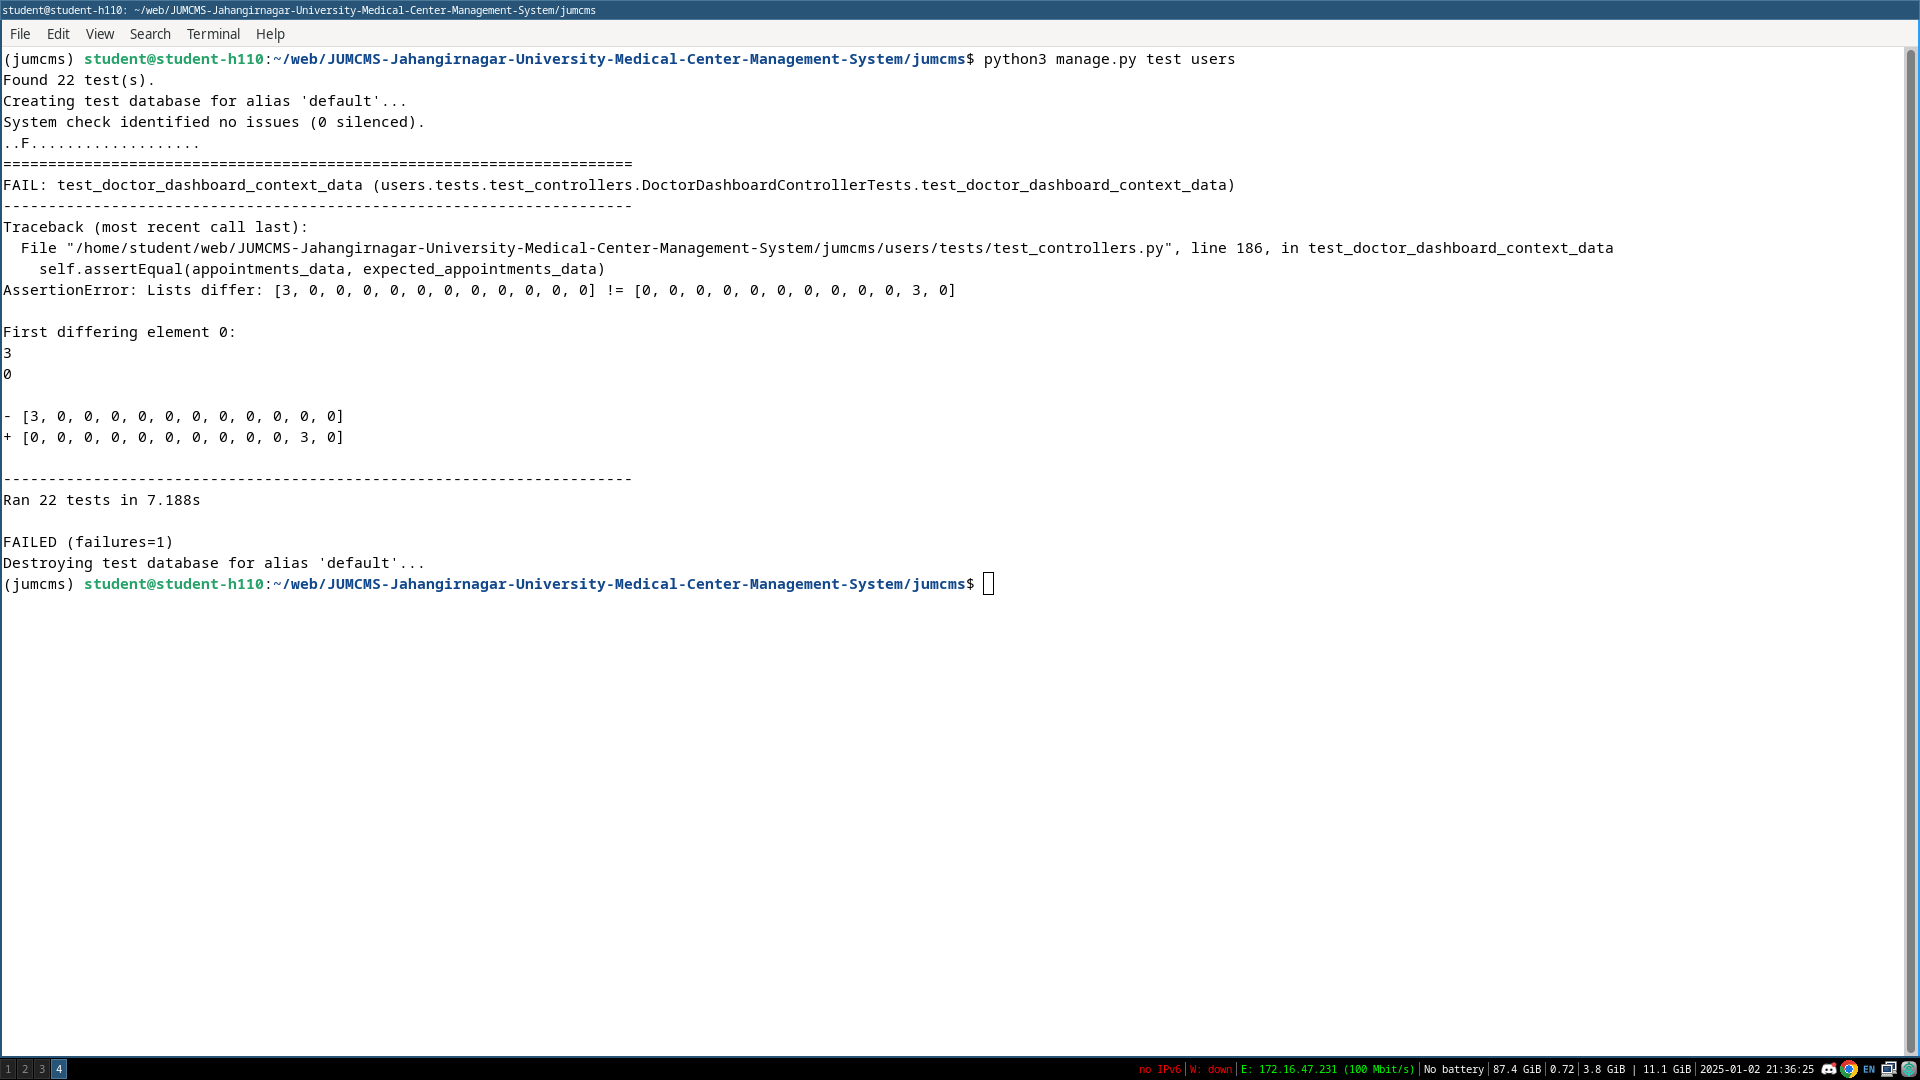
\includegraphics[width=1\textwidth]{images/test1.png}
    \caption{Test Case Passed}
    \label{fig:testcreateaccount}
\end{figure}
\subsection{Dispense Medicine to patients}
\textbf{Code for Dispense Medicine}
\lstset{style=pythonSolarized}
\begin{lstlisting}

@login_required
def dispense_medicines(request, prescription_id):
    """
    Dispense medicines to patient
    :param: request, int
    :return: html
    """
    if request.user.role != "Storekeeper":
        return HttpResponseForbidden("You are not authorized to view this page.")
    if request.method == "POST":
        prescription = get_object_or_404(Prescription, id=prescription_id)
        prescribed_medicines = PrescribedMedicine.objects.filter(
            prescription=prescription
        )
        medicines_info = []
        for prescribed_medicine in prescribed_medicines:
            medicine = prescribed_medicine.medicine
            required_quantity = (
                prescribed_medicine.duration
            )  # Assuming the duration is the quantity needed
            in_stock = medicine.stock_quantity

            # Check if the stock is sufficient
            is_stock_sufficient = in_stock >= required_quantity

            if is_stock_sufficient:
                medicine.stock_quantity -= required_quantity
                medicine.save()
                medicines_info.append(
                    {
                        "medicine_name": medicine.name,
                        "required_quantity": required_quantity,
                        "in_stock": in_stock,
                        "is_stock_sufficient": is_stock_sufficient,
                        "frequency": prescribed_medicine.dosage_frequency,
                        "instructions": prescribed_medicine.instructions,
                    }
                )

        if medicines_info:
            messages.success(request, f"dispensed successfully.")
            pdf_response = generate_pdf(
                medicines_info,
                prescription.doctor_appointment.doctor.user.name,
                prescription.doctor_appointment.patient.user.name,
                prescription_id,
            )
            return pdf_response

        else:
            messages.error(request, f"Not enough stock.")
            return redirect("medicines:search-prescriptions")
    else:
        return redirect("medicines:prescription-details", prescription_id)


\end{lstlisting}
\textbf{Test Case Dispense Dedicine}
\lstset{style=pythonSolarized}
\begin{lstlisting}
    @patch("medicines.controllers.generate_pdf")  # Mock the generate_pdf function
    def test_dispense_medicines_view_success(self, mock_generate_pdf):
        """
        Test dispense_medicines_view_success
        :param mock_generate_pdf:
        :return:
        """
        mock_generate_pdf.return_value = HttpResponse()  # Mock the return value

        self.client.force_login(self.storekeeper_user)
        response = self.client.post(
            reverse("medicines:dispense-medicines", args=[self.prescription.id])
        )

        # Assert that the medicine stock quantity is updated
        updated_medicine = Medicine.objects.get(id=self.medicine.id)
        self.assertEqual(updated_medicine.stock_quantity, 95)

        # Assert that the response is a redirect (since generate_pdf is mocked)
        self.assertEqual(response.status_code, 200)

    def test_dispense_medicines_view_not_enough_stock(self):
        """
        test dispense medicines view_not_enough_stock
        :return: Boolean
        """
        self.client.force_login(self.storekeeper_user)
        self.medicine.stock_quantity = 2
        self.medicine.save()
        response = self.client.post(
            reverse("medicines:dispense-medicines", args=[self.prescription.id])
        )

        self.assertEqual(response.status_code, 302)
        self.assertEqual(response.url, reverse("medicines:search-prescriptions"))


\end{lstlisting}
\begin{figure}[H]
    \centering
    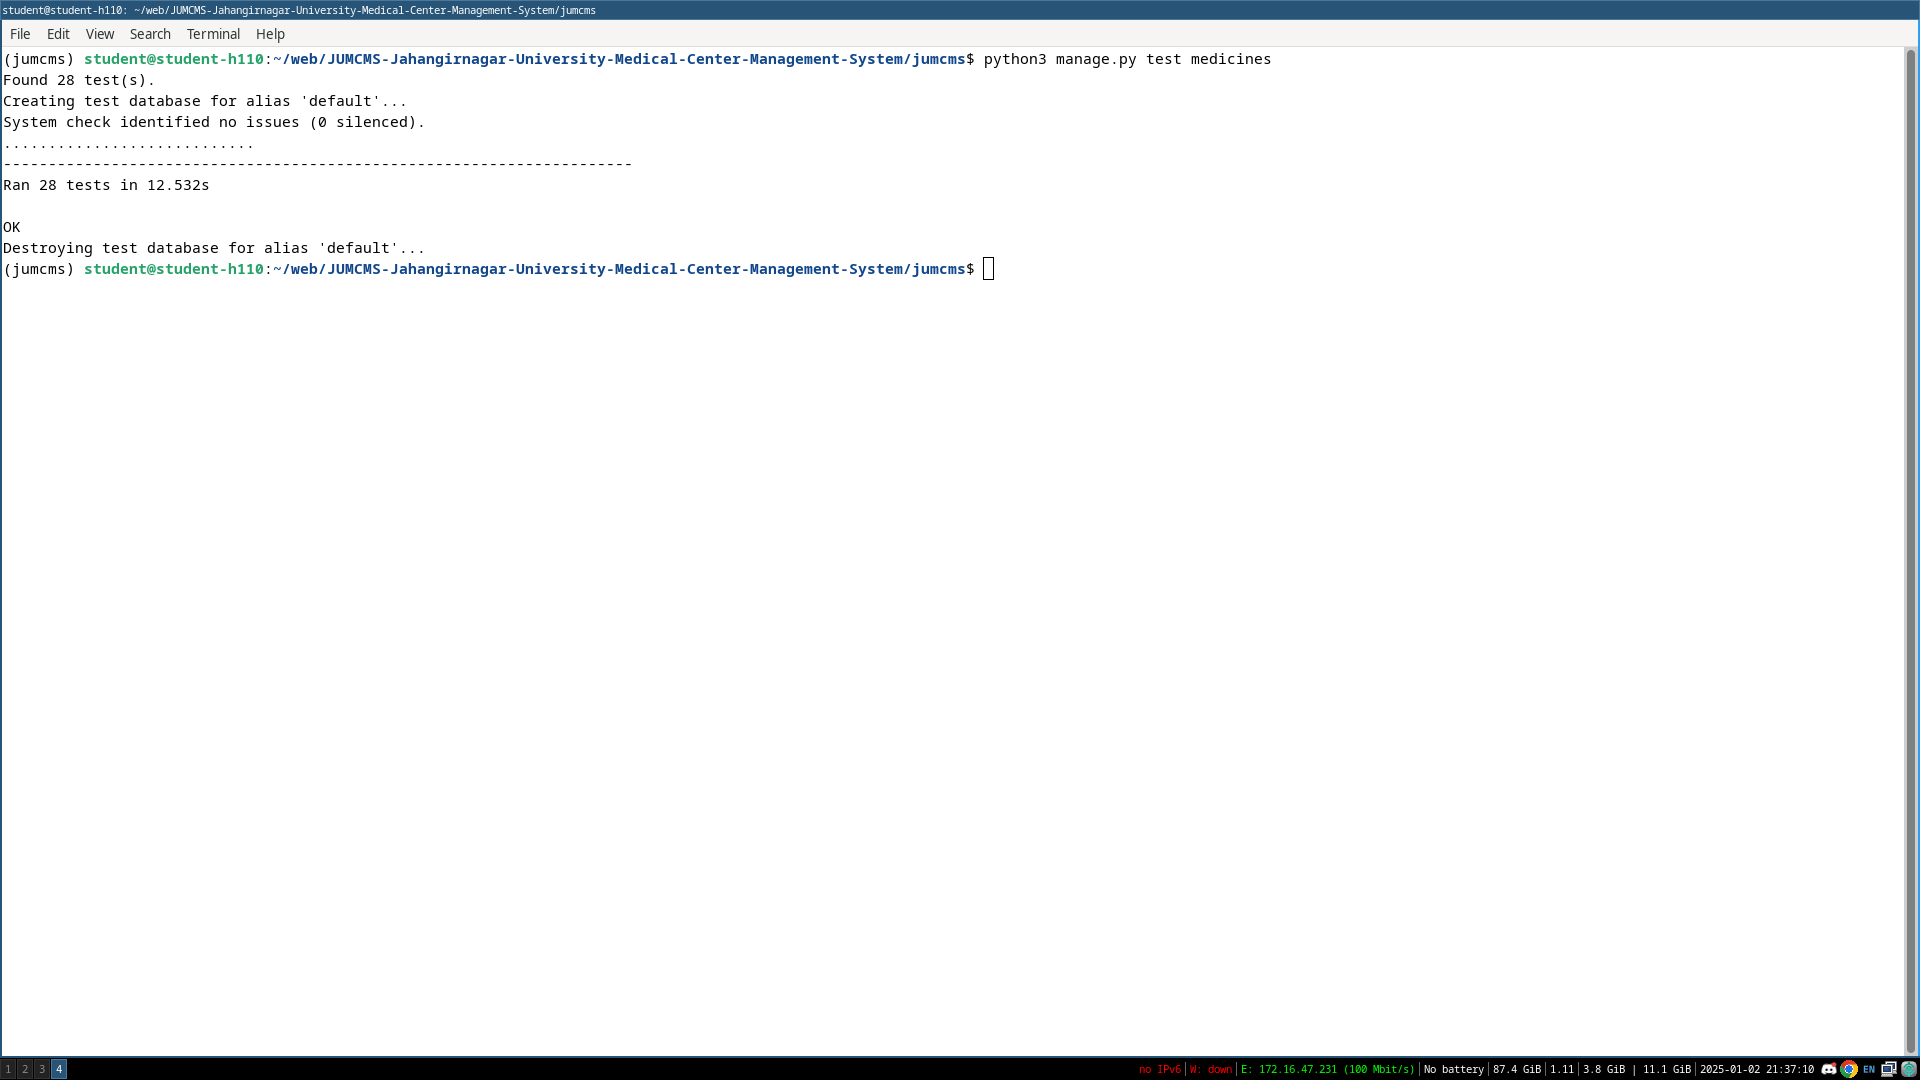
\includegraphics[width=1\textwidth]{images/test2.png}
    \caption{Test Case Passed}
    \label{fig:testdispense}
\end{figure}

\subsection{Update Stock information}
\textbf{Code for Update Stock information}
\lstset{style=pythonSolarized}
\begin{lstlisting}
@login_required
def add_medicine(request):
    if request.user.role != "Storekeeper":
        return HttpResponseForbidden("You are not authorized to view this page.")
    user = request.user
    if request.method == "POST":
        form = MedicineForm(request.POST)
        if form.is_valid():
            form.save()
            return redirect(
                "users:storekeeper_dashboard"
            )  # Replace with your actual success URL
    else:
        form = MedicineForm()
    return render(
        request, "storekeeper/add_medicine.html", {"form": form, "user": user}
    )


\end{lstlisting}
\textbf{Test Case for Update Stock Information}
\lstset{style=pythonSolarized}
\begin{lstlisting}
    def test_add_medicine_controller(self):
        """
        Test add_medicine_controller

        """
        self.client.force_login(self.storekeeper_user)
        self.assertEqual(Medicine.objects.count(), 1)
        response = self.client.post(
            reverse("medicines:add-medicine"),
            {
                "name": "Capa",
                "generic_name": "Maracetamol",
                "manufacturer": "Square",
                "dosage_form": "Tablet",
                "strength": "200mg",
                "description": "Used for fever",
                "price": 10.00,
                "stock_quantity": 100,
                "expiry_date": "2025-12-31",
            },
            follow=False,
        )
        self.assertRedirects(response, reverse("users:storekeeper_dashboard"))
        self.assertEqual(response.status_code, 302)
        self.assertEqual(Medicine.objects.count(), 2)
        self.assertEqual(Medicine.objects.first().name, "Paracetamol")
        self.assertEqual(Medicine.objects.first().generic_name, "Acetaminophen")
        self.assertEqual(Medicine.objects.first().manufacturer, "ABC Pharma")
        self.assertEqual(Medicine.objects.first().dosage_form, "Tablet")
        self.assertEqual(Medicine.objects.first().strength, "500mg")
        self.assertEqual(Medicine.objects.first().description, "Pain reliever")
        self.assertEqual(Medicine.objects.first().price, 10.00)
        self.assertEqual(Medicine.objects.first().stock_quantity, 100)
        self.assertEqual(str(Medicine.objects.first().expiry_date), "2025-12-31")


\end{lstlisting}

\begin{figure}[H]
    \centering
    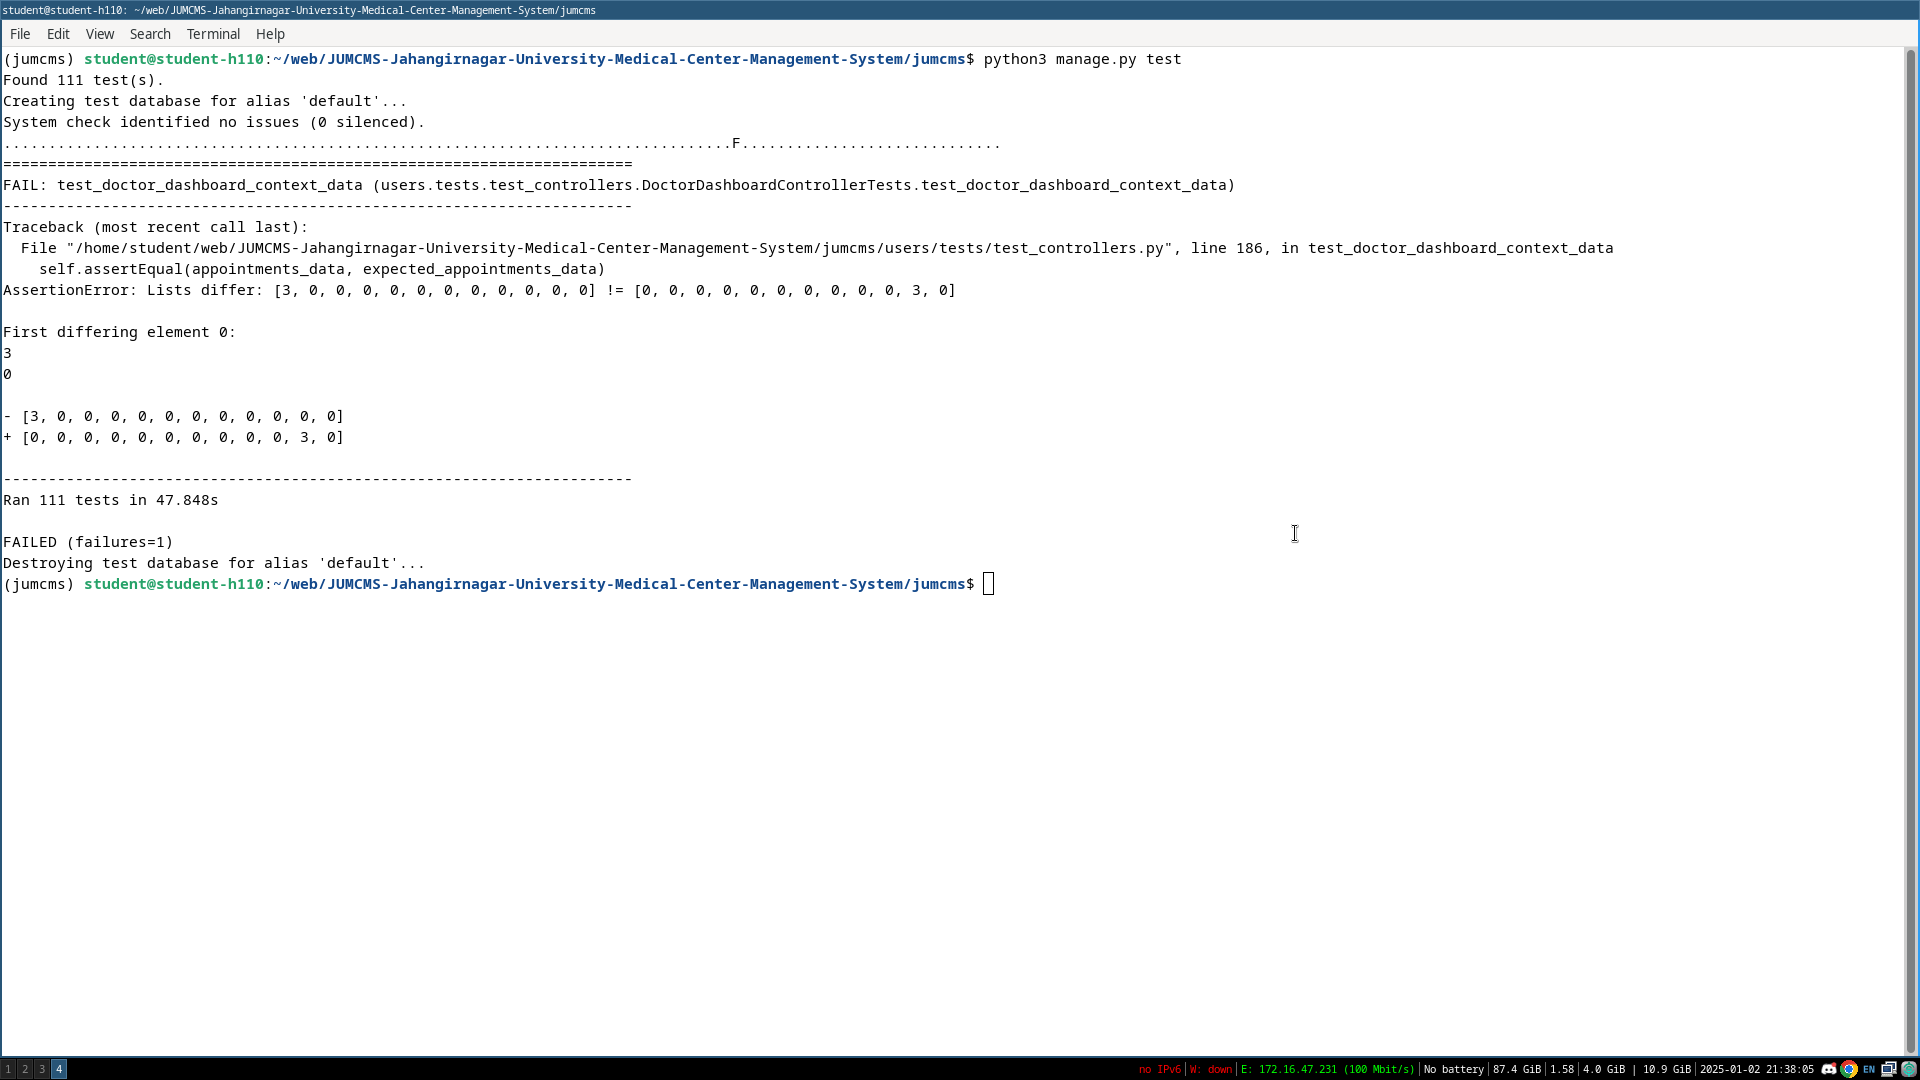
\includegraphics[width=1\textwidth]{images/test3.png}
    \caption{Test Case Passed}
    \label{fig:testupdatestock}
\end{figure}
\section{Pros and Cons of Unit Testing}
\subsection{Pros}
\begin{enumerate}
    \item Improved Code Quality:
        \begin{itemize}
            \item Ensures each function works as expected.
            \item Helps identify bugs early in the development cycle.
            \item Example: In the Bangla Sign Language Recognition project, unit testing helped validate preprocessing steps for image data, ensuring consistent input to the model.
        \end{itemize}
    \item Facilitates Refactoring:
        \begin{itemize}
            \item Unit tests act as a safety net when modifying existing code.
            \item Example: When optimizing database queries in the medical center system, unit tests ensured that no existing functionality broke during refactoring.
        \end{itemize}
    \item Documentation:
        \begin{itemize}
            \item Unit tests serve as live documentation for the expected behavior of functions.
        \end{itemize}

    \item Cost-Effective in the Long Run:
        \begin{itemize}
            \item Early detection of bugs saves time and resources in debugging and maintenance.
        \end{itemize}
\end{enumerate}
\subsection{Cons}
\begin{enumerate}
    \item Time-Consuming:
        \begin{itemize}
            \item  Writing and maintaining unit tests require significant effort.
            \item Example: During the affordable housing app development, creating unit tests for all functionalities consumed a large portion of the initial development timeline.
        \end{itemize}
    \item Doesn’t Catch Integration Issues:
        \begin{itemize}
            \item Unit testing focuses on individual components, not their interactions.
            \item Example: In the sign language project, unit tests didn’t catch errors in the video data pipeline’s integration with the Flask backend.
        \end{itemize}
    \item Overhead in Rapid Prototyping:
        \begin{itemize}
            \item In early-stage projects, the overhead of writing unit tests can delay feature delivery.
        \end{itemize}
\end{enumerate}
\section{Impact of Unit Testing on Project Outcomes}
\begin{enumerate}
    \item Enhanced Reliability:
        \begin{itemize}
 \item Unit tests improve software reliability by catching edge cases early.
 \item Example: Automated tests in the Sudoku game app detected invalid board setups, ensuring the app provided consistent user experiences.
 \end{itemize}
 \item Collaboration and Code Integration:
     \begin{itemize}
 \item Encourages modular code design and smoother integration of team members’ work.
 \item Example: In the medical center project, each team member worked on separate modules, tested independently using unit tests, and integrated seamlessly.
 \end{itemize}
 \item Supports Agile Practices:
     \begin{itemize}
 \item Unit testing complements TDD and continuous integration by providing fast feedback.
 \item Example: In Sprint 2, unit testing was essential for validating new features like the notifications module.
 \end{itemize}
 \item Challenges with Some Practices:
     \begin{itemize}
 \item Practices like exploratory coding can be incompatible with unit testing, as test cases are hard to define in unstructured code.
 \item Example: During initial prototype development in the affordable housing app, testing was deferred to prioritize rapid iteration.
 \end{itemize}
\end{enumerate}
\section{Recommended Guidelines for Good Practices with Unit Testing}
\begin{enumerate}

    \item Adopt TDD to define tests before implementation.
    \item Ensure all critical paths and edge cases are tested.
    \item Test one functionality per test case.
    \item Use CI/CD pipelines to run tests automatically after each code commit.
    \item Update tests as code evolves to maintain relevance.
    \item Mock dependencies to isolate the unit under test.
    \item Example: Mocking the database connection in inventory management tests prevented test failures due to external system issues.
    \item Educate team members about the importance and techniques of unit testing.
\end{enumerate}
\section{Conclusion}
Unit testing is a vital practice for ensuring software reliability and maintainability. While it requires an
initial investment of time and effort, its long-term benefits in improving code quality, facilitating
collaboration, and supporting agile practices outweigh the challenges. By adopting recommended practices and
leveraging real-world lessons, teams can maximize the effectiveness of unit testing in their projects.
\end{document}
